\begin{frame}{Experiments and Numerical Analysis}
    \begin{columns}
        \begin{column}{.6\textwidth}
            \centering
            \textbf{Applications to both 1D and 2D cases} \\
            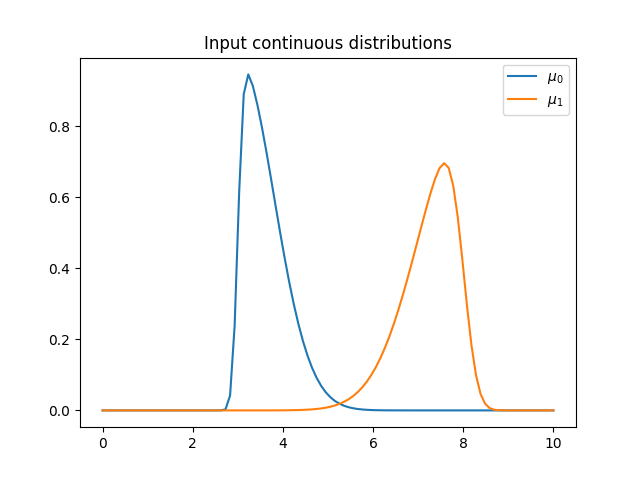
\includegraphics[height=.35\textheight]{figures/1D_inputs.png} \\
            Continuous skewed normal distributions
            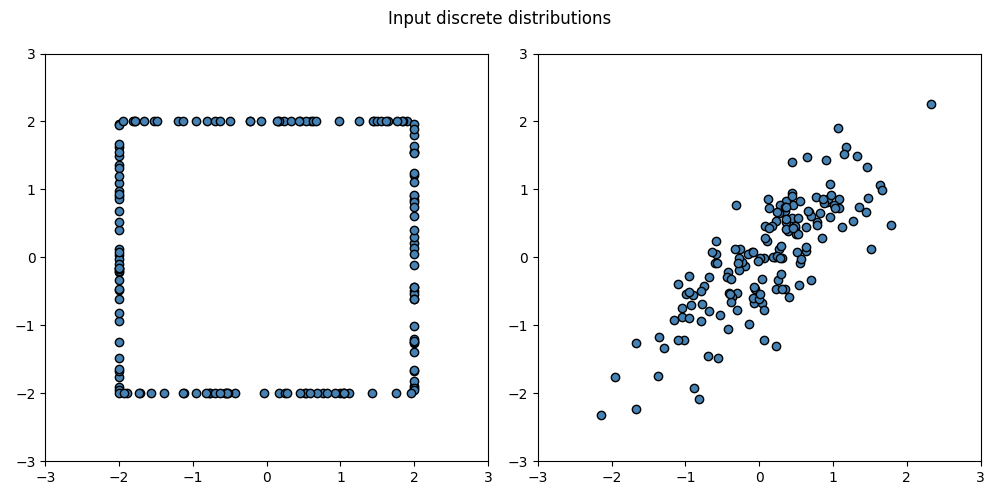
\includegraphics[height=.35\textheight]{figures/2D_inputs.png} \\
            Discrete uniform distributions
        \end{column}
        \begin{column}{.4\textwidth}
        \textbf{Comparison to existing methods} 
        \begin{itemize}
            \item McCann's interpolation
            \item Iterative Sinkhorn algorithm
            \item Free support Sinkhorn algorithm \parencite{cuturi_fast_2014} from POT toolbox \parencite{flamary_pot_2021}
        \end{itemize}
        \end{column}
    \end{columns}
\end{frame}

\begin{frame}{Experiment 1}
    \centering
    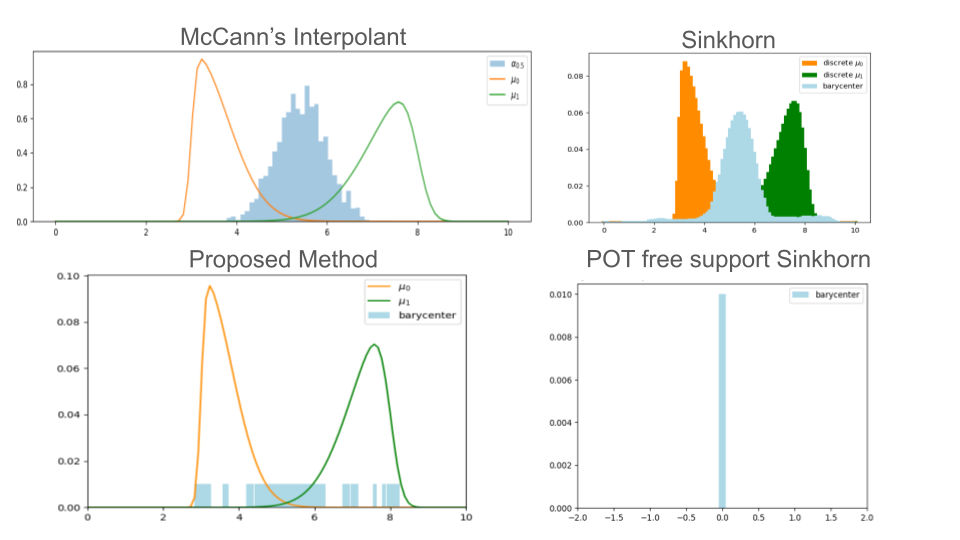
\includegraphics[width=\textwidth]{figures/experiment1_results.png}
\end{frame}

\begin{frame}{Experiment 2}
    \centering
    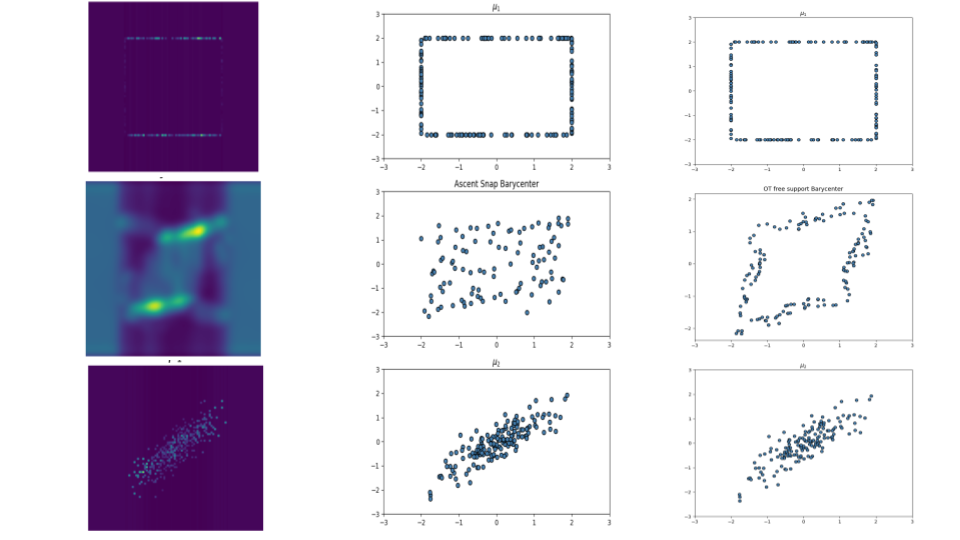
\includegraphics[width=\textwidth]{figures/experiment2_results.png}
    Sinkhorn Algorithm (left), Proposed method (middle), Free support Sinkhorn using POT (right)
\end{frame}

\begin{frame}{Computation time}
    \begin{table}
        \begin{center}
            \begin{tabularx}{\textwidth}{>{\raggedright}m{2cm} c m{2cm} X X}
                    Experiment & McCann & Iterative Bregman & POT free support & Ascent Snap \\
                    \hline\hline
                    1D skewnorm & $0.02 \pm 0.01$ & $0.22 \pm 0.02$ & $0.74 \pm 0.28$ & $7814.27 \pm 0.37$ \\
                    2D discrete & - & $2.18 \pm 0.34$ & $0.38 \pm 0.30$ & $16351.66 \pm 0.23$ \\
            \end{tabularx}
        \end{center}
        \caption{Computation time (in seconds) for the different methods. The experiments were conducted three times for the Ascent snap algorithm and ten times for the others.}
    \end{table}
\end{frame}

\begin{frame}{Ascent step convergence}
    \begin{figure}
    \begin{columns}
        \begin{column}{.5\textwidth}
            \begin{subfigure}{\textwidth}
            \centering
            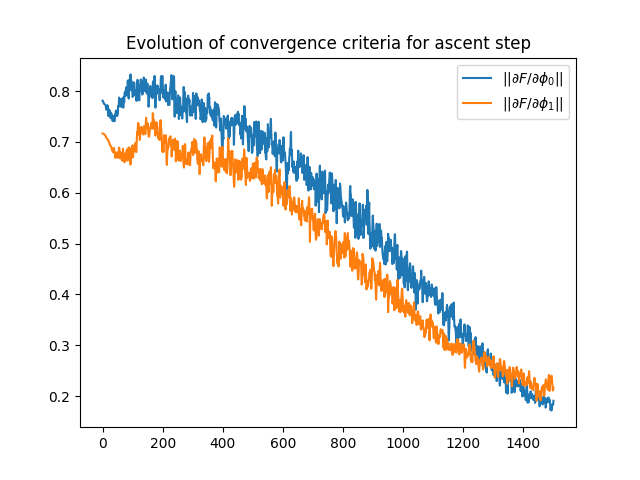
\includegraphics[width=\textwidth]{figures/ascent_criteria_msamples16000_iter0_1D_2skewnorm.png}
            \caption{Two 1D continuous distributions}
            \end{subfigure}
        \end{column}
        \begin{column}{.5\textwidth}
            \begin{subfigure}{\textwidth}
                \centering
                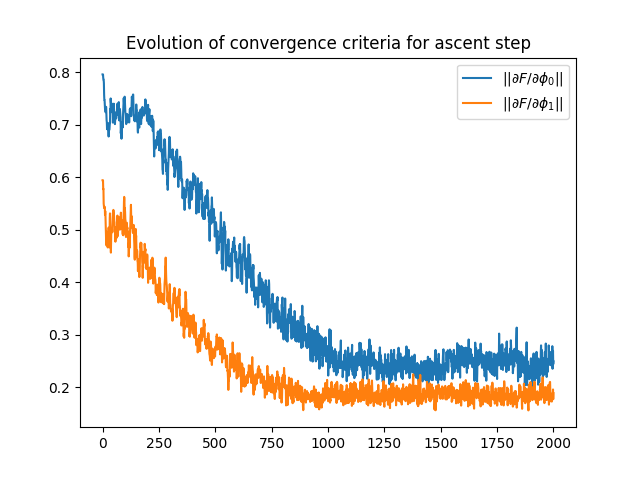
\includegraphics[width=\textwidth]{figures/ascent_criteria_msamples16000_iter0_2D_discrete.png}
                \caption{Two 2D discrete distributions }
            \end{subfigure}
        \end{column}
    \end{columns}
    \caption{\centering Evolution of $\norm{ \frac{\partial F}{\partial \phi_j} }$ during the ascent step for each experiment. In the x-axis, is the number of interations of the while loop.}
    \end{figure}
\end{frame}

\begin{frame}{Ascent step time}
    \begin{table}
        \begin{center}
                \begin{tabular}{lrr}
                        Experiment & Ascent step & Snap step \\
                        \hline\hline
                        1D skewnorm & $8309.44 \pm 0.33$ & $5.28 \pm 0.23$ \\
                        2D discrete & $11938.70 \pm 0.34$ & $9.81 \pm 0.34$ \\
                \end{tabular}
        \end{center}
        \caption{Computation time (in seconds) for each step of the proposed algorithm. The experiences were repeated $3$ times.}
        \label{table:time_algo_table}
    \end{table}
\end{frame}